\section{Result Report}
\label{sec:analyze_results}

When a run completes, the Analyze task produces a result report similar in shape to the Evaluation report (see \nameref{sec:eval}). The report appears in the Flight Deck 'Reports' panel and can be exported from there. \\

The result tree is structured as:

\begin{itemize}
\item Overview: combined dataset summary, selected Data Sources, RefTraj reference, license tier
\item One top-level section per executed inspector
\begin{itemize}
\item Data Item Inspection: per-DS, per-CAT cumulative tables
\item Sensor Coverage and PD: the three projections plus a numeric summary
\item Position Accuracy: reported / offset / consistency subsections, plus per-source repeats where applicable
\item RU Coverage: per-RU and Dominant RU subsections
\item RU Effect: marginal effect table, redundancy curve and per-RU drill-down subsections
\end{itemize}
\end{itemize}
\ \\

\begin{figure}[H]
  \centering
  \hspace*{-2.5cm}
    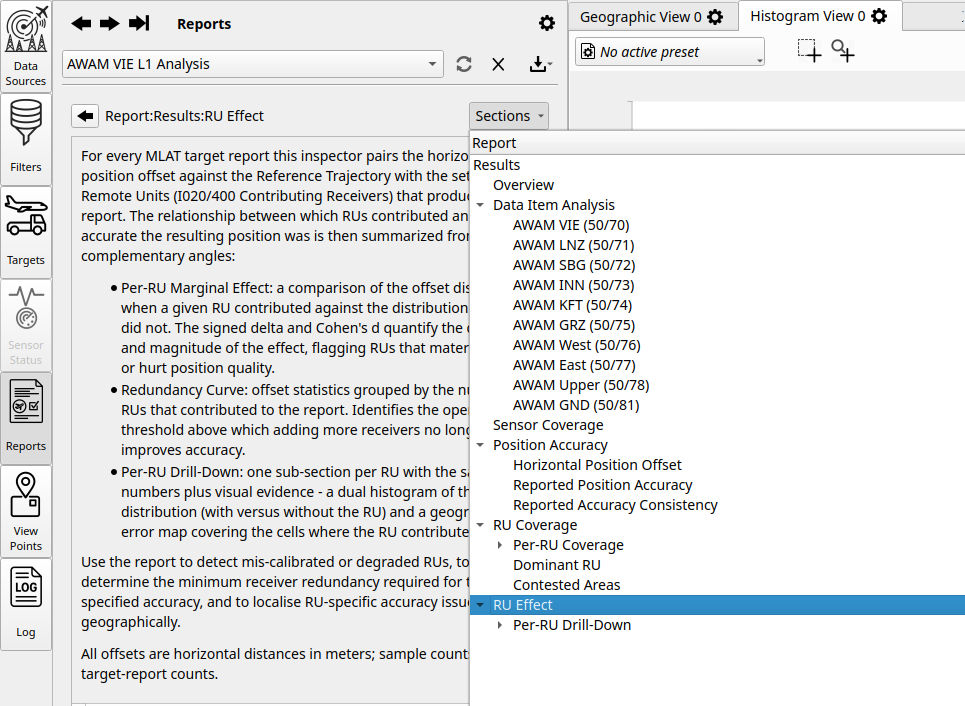
\includegraphics[width=19cm,frame]{figures/analyze_mlat_report.png}
  \caption{Analyze result report tree}
\end{figure}

